%%%%%%%%%%%%%%%%%%%%%%%%%%%%%%%%%%%%%%%%%
% University/School Laboratory Report
% LaTeX Template
% Version 3.0 (4/2/13)
%
% This template has been downloaded from:
% http://www.LaTeXTemplates.com
%
% Original author:
% Linux and Unix Users Group at Virginia Tech Wiki 
% (https://vtluug.org/wiki/Example_LaTeX_chem_lab_report)
%
% License:
% CC BY-NC-SA 3.0 (http://creativecommons.org/licenses/by-nc-sa/3.0/)
%
%%%%%%%%%%%%%%%%%%%%%%%%%%%%%%%%%%%%%%%%%

%----------------------------------------------------------------------------------------
%	PACKAGES AND DOCUMENT CONFIGURATIONS
%----------------------------------------------------------------------------------------

\documentclass{article}

\usepackage{graphicx} % Required for the inclusion of images

\setlength\parindent{0pt} % Removes all indentation from paragraphs

%\usepackage{times} % Uncomment to use the Times New Roman font

%----------------------------------------------------------------------------------------
%	DOCUMENT INFORMATION
%----------------------------------------------------------------------------------------

\title{Barobo Linkbot USB and Main Motherboard Flashing Jigs \\ User Guide} % Title

\author{David \textsc{Ko}} % Author name

\date{\today} % Date for the report

\begin{document}

\maketitle % Insert the title, author and date

\section{Procedure for Flashing and Testing Linkbots Motherboards}
\begin{enumerate}
\item Disconnect all usb devices from the computer, except for critical devices
   such as keyboards and mice.
\item Using a mini-USB cable, connect the Pololu PGM03A programming on the jig to
   the computer. Red and yellow lights should begin flashing on the programmer.
   The PGM03A creates two tty devices on the Linux system: \texttt{/dev/ttyACM0} and
   \texttt{/dev/ttyACM1} . \texttt{/dev/ttyACM0} is the device that represents the programmer.

   \begin{center}
   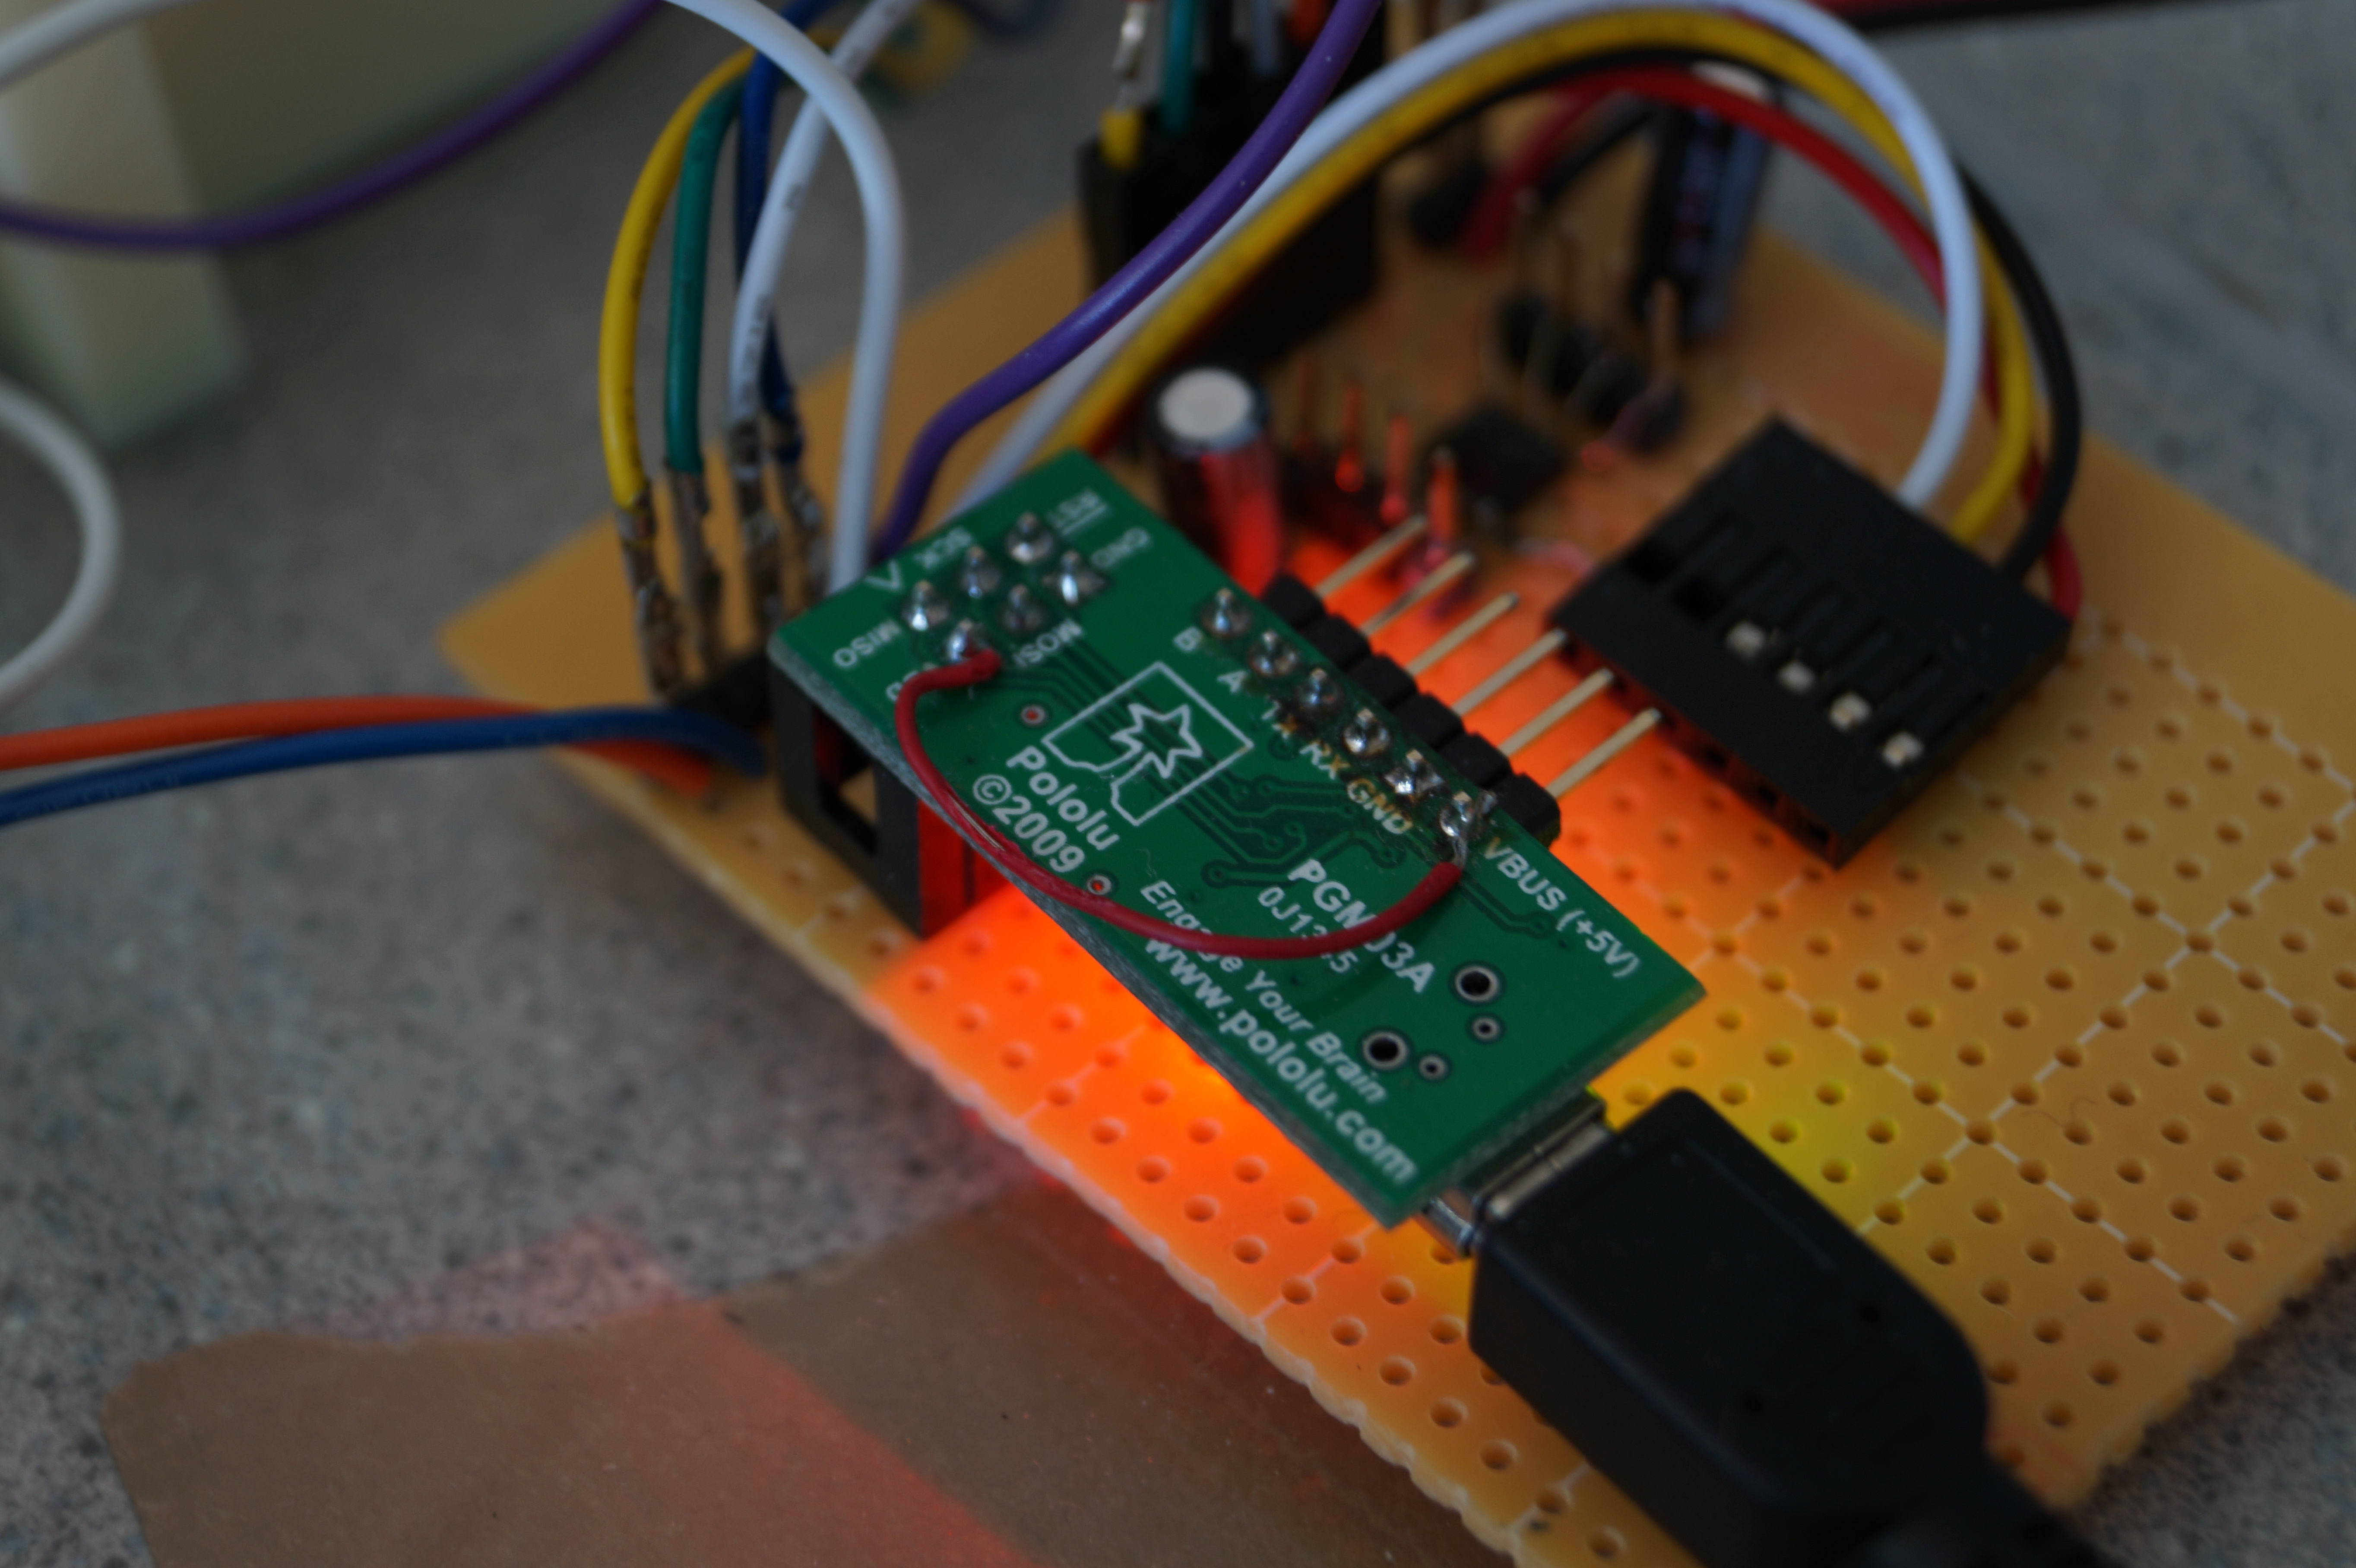
\includegraphics[width=4in]{images/programmer.jpg}
   \end{center}

\item Using a micro-USB cable, connect a powered-on Linkbot to the computer. The
   Linkbot should create an additional tty device at \texttt{/dev/ttyACM2}.
\item Start the program ``BaroboFirmwareLoader.py'' by double clicking on it.
\item In the BaroboFirmwareLoader utility, select \texttt{/dev/ttyACM2} as the Dongle
   port and click ``Connect'' in the ``Dongle Management'' area of the dialog. 

   Select \texttt{/dev/ttyACM0} as the programmer port.
\item Using an additional micro-USB cable, connect a Linkbot "ILW" usb board to
   the computer.

   \begin{center}
   \includegraphics[width=4in]{images/usb_board.jpg}
   \end{center}

\item \label{restartstep}Connect the motherboard to be flashed to the Linkbot USB board. Make sure
   that all twelve pins on the USB board correctly go into all twelve holes on
   the motherboard.

   \begin{center}
   \includegraphics[width=4in]{images/usb_pins.jpg}
   \end{center}

\item Power on the board by pressing and holding the power button on the USB board
   until the board turns on (The small LED on the USB board should change from
   purple to blue).

   \begin{center}
   \includegraphics[width=2in]{images/usb_purple.jpg}
   \includegraphics[width=2in]{images/usb_blue.jpg}
   \end{center}

\item Affix the motherboard to the jig. 

   \begin{center}
   \includegraphics[width=4in]{images/motherboard_jig.jpg}
   \end{center}

\item On the BaroboFirmwareLoader utility, click on the button labeled "Flash
  and Test Board". Avoid touching components other than the phone-jack on the
  motherboard during the flashing process.
\item A progress bar should appear indicating that the board is being flashed. 
  After the board is flashed, a randomly generated serial ID is programmed onto 
  the board and the testing procedure automatically begins.
\item During the testing procedure, the dongle Linkbot connects wirelessly to
  the motherboard. The dongle instructs the motherboard to spin the motors in the
  positive direction, play a low, high, and low tone with the buzzer, and reads
  the accelerometer data. This ensures that the wireless radio, motors, buzzer, and
  accelerometer are all working.
  \begin{itemize}
    \item If the test should fail, an error dialog will pop up attempting to
    describe the nature of the failure. The test may be re-run by clicking on
    the ``Run Test Routine'' button. This causes the utility to run only the
    test routine, bypassing the reflashing process. If the test routine fails
    more than once, it may be an indication of a bad motherboard.
  \end{itemize}
\item \label{stopstep} Once the test routine is finished, the usb board may be removed from the
  motherboard and steps \ref{restartstep} through
  \ref{stopstep} may be repeated to flash additional motherboards.
\end{enumerate}

\section{Procedure for Flashing and Testing Linkbots USB Boards}

\begin{enumerate}
\item Attach the USB jig to the computer using a Mini-USB cable.

   \begin{center}
   \includegraphics[width=4in]{images/usb_jig.jpg}
   \end{center}

\item Start the program ``BaroboUSBFirmwareLoader'' by double clicking on the icon.

\item \label{usbjig_step_begin} Affix the new USB board to be flashed onto the jig, making sure the pins
on the jig line up with pads on the USB board. When it is correctly seated, a
red light should turn on on the USB board.

   \begin{center}
   \includegraphics[width=2in]{images/usb_jig_pins.jpg}
   \includegraphics[width=2in]{images/usb_jig_loaded.jpg}
   \end{center}

\item \label{usbjig_step_stop} Click on the button labeled ``Flash Linkbot USB Board''. A progress
dialog box will be shown. If everything flashes correctly, the dialog box will
close. Otherwise, an error message will be displayed.

\item Steps \ref{usbjig_step_begin} through \ref{usbjig_step_stop} may be repeated to flash additional boards.
\end{enumerate}

\end{document}
